    \chapter{绿色化学与工业过程}\label{ch:b3:green-industrial}

布洛芬过去需要六步合成，各步丢弃的质量都多于保留的质量：
每生产一千克药物，铝盐、氯化钠、乙醇、氨和乙酸都要离开工厂。
自 1992 年起，一条三步催化路线使所用原子的大部分
进入产物，其唯一的副产物乙酸被回收并出售。
本章用数字比较此类过程，包括\omterm{def:b3:green-industrial:atom-economy}{原子经济性}、E 因子和\omterm{def:b3:green-industrial:pmi}{过程质量强度}；
随后讨论溶剂、能量与\omterm{def:b3:green-industrial:lca}{生命周期评价}，
以及一些大型化工过程如何变得更清洁，
还有\omterm{def:b3:green-industrial:feedstock}{可再生原料}
与酶会带来怎样的改变。

\begin{recall}
第 1 册介绍了\omterm{def:b3:green-industrial:atom-economy}{原子经济性}和\omterm{def:b3:green-industrial:green-chemistry}{绿色化学}；本科一年级分册讨论了
产率；本科二年级分册讨论了反应器、转化率、选择性、停留时间、
单程转化率、循环与驰放、绝热温升、
电解槽和燃料电池。\Cref{ch:b3:surfaces-catalysis}和
\cref{ch:b3:homogeneous-catalysis}讨论了催化，
\cref{ch:b3:total-synthesis}讨论了合成路线的衡量指标。
\end{recall}

\begin{omfigure}
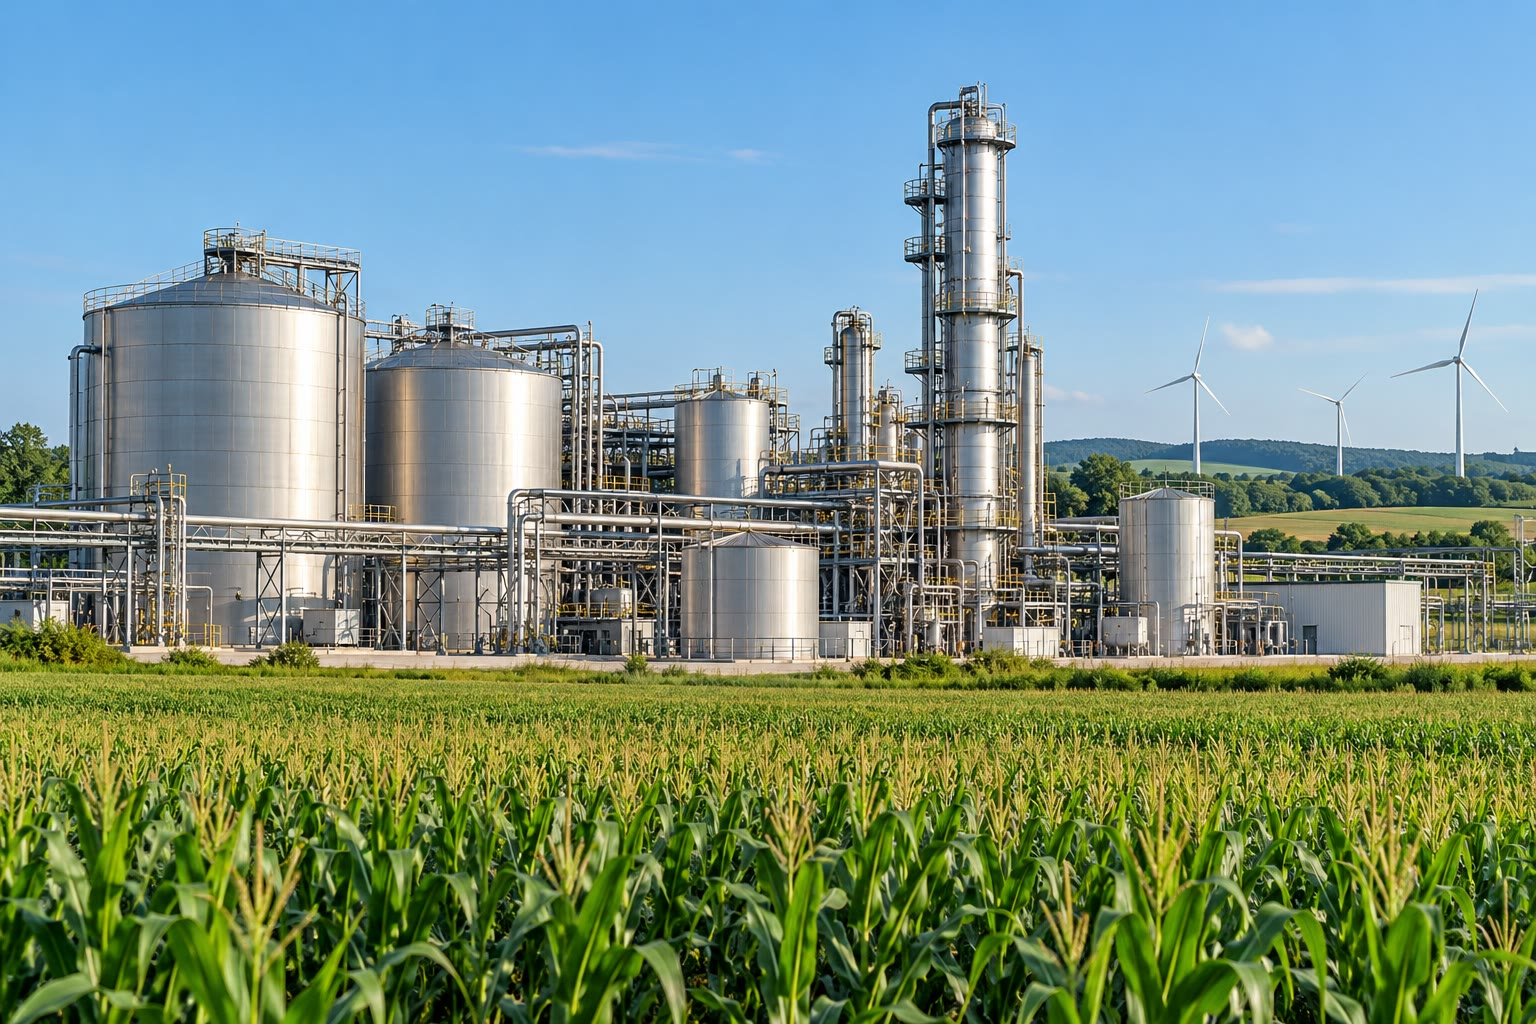
\includegraphics[width=0.58\linewidth]{images/book4/ai/b3-31-biorefinery.jpg}

{\small 生物精炼厂：发酵罐和蒸馏塔，将作物
与残余物转化为燃料和平台化学品。}
\end{omfigure}

\section{绿色程度的衡量}

\begin{definition}[绿色化学]\label{def:b3:green-industrial:green-chemistry}
称\emph{绿色化学}\index{绿色化学}为一类化学产品与过程的设计，
其目的在于减少或消除有害物质的
使用和产生，可概括为十二条原则：防止废物产生、
最大化\omterm{def:b3:green-industrial:atom-economy}{原子经济性}、使用和制造危害较小的物质、设计更安全的产品、
使用更安全的溶剂、节约能源、使用\omterm{def:b3:green-industrial:feedstock}{可再生原料}、避免不必要的
衍生化、优先使用催化剂而非化学计量试剂、为降解而设计、
实时监测，并选择本质更安全的化学。
\end{definition}

\begin{definition}[原子经济性]\label{def:b3:green-industrial:atom-economy}
反应的\emph{原子经济性}\index{原子经济性}是指目标产物的摩尔质量
与平衡化学方程式中全部反应物摩尔质量之和的比，
以百分数表示。
\end{definition}

\begin{proposition}[按反应类型划分的原子经济性]\label{prop:b3:green-industrial:ae-classes}
加成反应与重排反应的\omterm{def:b3:green-industrial:atom-economy}{原子经济性}为 100\,\%；取代反应和
消除反应则较低。
\end{proposition}

\begin{proof}
在加成反应 $\mathrm{A} + \mathrm{B} \to \mathrm{AB}$ 或重排反应 $\mathrm{A} \to \mathrm{A'}$ 中，唯一的产物包含全部
反应物的原子，因此其摩尔质量等于它们之和。
取代反应 $\mathrm{A{-}X} + \mathrm{Y} \to \mathrm{A{-}Y} + \mathrm{X}$ 或消除反应 $\mathrm{A} \to \mathrm{B} + \mathrm{C}$ 会生成
第二种产物，它带走了一部分质量。
\end{proof}

\begin{definition}[E 因子]\label{def:b3:green-industrial:e-factor}
过程的\emph{E 因子}\index{E 因子}是指每单位产物质量所产生的
废物质量。在完整 E 因子中，凡未进入产物的投入均计为
废物，包括溶剂和水；简单 E 因子则不计溶剂和
水。
\end{definition}

\begin{definition}[过程质量强度]\label{def:b3:green-industrial:pmi}
\emph{过程质量强度}\index{过程质量强度}（PMI）是指
投入一个过程的物料总质量（反应物、试剂、溶剂、
水）与产物质量之比。
\end{definition}

\begin{proposition}[PMI 与 E 因子]\label{prop:b3:green-industrial:pmi-e}
在相同边界下，$\mathrm{PMI} = E + 1$，其中 $E$ 为完整 E 因子。
\end{proposition}

\begin{proof}
由质量守恒，投入的全部物质要么成为产物，要么成为废物：
$m_{\mathrm{in}} = m_{\mathrm{product}} + m_{\mathrm{waste}}$。除以 $m_{\mathrm{product}}$ 得 $\mathrm{PMI} = 1 + E$。
\end{proof}

\begin{definition}[反应质量效率]\label{def:b3:green-industrial:rme}
\emph{反应质量效率}\index{反应质量效率}（RME）是指一个反应
所得产物质量与所用全部
反应物质量之比。
\end{definition}

\begin{proposition}[由产率和原子经济性求 RME]\label{prop:b3:green-industrial:rme}
$\mathrm{RME} = \mathrm{AE} \times \text{产率}/\mathrm{SF}$，其中化学计量因子 $\mathrm{SF} \ge 1$ 为所用
反应物质量与配平方程式所需质量之比。
\end{proposition}

\begin{proof}
若预期生成一摩尔产物，方程式需要质量为 $\sum M_r$ 的反应物，
实际反应使用 $\mathrm{SF}\sum M_r$，得到的产物质量为 $\text{产率} \times M_{\mathrm p}$。相除得：
$\mathrm{RME} = \text{产率}\,M_{\mathrm p}/(\mathrm{SF}\sum M_r) = \mathrm{AE} \times \text{产率}/\mathrm{SF}$。
\end{proof}

\begin{method}[计算路线的各项指标]\label{met:b3:green-industrial:metrics}
\begin{enumerate}
  \item 写出每一步的配平方程式，并由进入路线的全部反应物计算
        路线的\omterm{def:b3:green-industrial:atom-economy}{原子经济性}。
  \item 由批次记录，将投入的全部物料质量相加（反应物、
        试剂、溶剂、水、后处理用料）：PMI = 投入总质量 / 产物质量。
  \item $E = \mathrm{PMI} - 1$；若回收与再利用的物流位于
        边界之内，应予扣除，并加以说明。
  \item 计算每一步的 RME：产物 / 反应物，以找出物料损失的位置
        （产率低、试剂过量或\omterm{def:b3:green-industrial:atom-economy}{原子经济性}差）。
\end{enumerate}
\end{method}

\begin{omfigure}
\begin{tikzpicture}
\begin{axis}[name=a, width=0.48\linewidth, height=5.4cm, ybar, bar width=14pt, ymin=0, ymax=110,
  xtick={1,2,3,4}, xticklabels={{布洛芬，6 步}, {布洛芬，3 步}, {EO，氯醇法}, {EO，直接氧化}},
  x tick label style={font=\scriptsize, rotate=25, anchor=north east}, ylabel={原子经济性 / \%},
  axis lines=left, tick label style={font=\scriptsize}, label style={font=\small},
  nodes near coords, nodes near coords style={font=\scriptsize, /pgf/number format/fixed, /pgf/number format/precision=0},
  enlarge x limits=0.18]
\addplot[fill=omMeth!55, draw=omMeth] table[x=i, y=AE] {figdata/out/bachelor-3-green-metrics.dat};
\end{axis}
\begin{axis}[at={(a.east)}, anchor=west, xshift=1.4cm, width=0.48\linewidth, height=5.4cm, ybar, bar width=14pt, ymin=0, ymax=3.4,
  xtick={1,2,3,4}, xticklabels={{布洛芬，6 步}, {布洛芬，3 步}, {EO，氯醇法}, {EO，直接氧化}},
  x tick label style={font=\scriptsize, rotate=25, anchor=north east}, ylabel={最小 E 因子},
  axis lines=left, tick label style={font=\scriptsize}, label style={font=\small},
  nodes near coords, nodes near coords style={font=\scriptsize, /pgf/number format/fixed, /pgf/number format/precision=2},
  enlarge x limits=0.18]
\addplot[fill=omThm!45, draw=omThm] table[x=i, y=Emin] {figdata/out/bachelor-3-green-metrics.dat};
\end{axis}
\end{tikzpicture}

{\small 布洛芬两条合成路线与环氧乙烷（EO）两条合成路线的\omterm{def:b3:green-industrial:atom-economy}{原子经济性}，
以及它们所允许的最小 E 因子（所有产率均为 100\,\%，不用溶剂）：
$E_{\min} = (1 - \mathrm{AE})/\mathrm{AE}$。实际 E 因子在产率低于 100\,\%、使用过量试剂和
溶剂时数值更大。}
\end{omfigure}

\section{溶剂与能量}

溶剂通常占精细化学品或药物生产过程
质量的最大部分。溶剂选择指南按安全、健康与
环境标准对其进行分级：水、乙醇、乙酸乙酯、2-甲基四氢呋喃
和苯甲醚被推荐使用；二氯甲烷、三氯甲烷、苯、己烷、
二甲基甲酰胺和 1,4-二氧六环应避免使用或禁用。水、
超临界二氧化碳（能溶解非极性化合物，减压后
不留残留物）以及无溶剂反应，
从源头上解决了这一问题。

\begin{method}[使用溶剂选择指南]\label{met:b3:green-industrial:solvent-choice}
\begin{enumerate}
  \item 列出溶剂须完成的任务：溶解反应物、在试剂存在下保持稳定、
        沸点适中、后处理时能与水分离。
  \item 优先从推荐类别中选取，并核对其危险说明。
  \item 若必须使用有问题的溶剂，则应寻找具有相同功能的推荐溶剂
        （如用 2-甲基四氢呋喃替代萃取中的二氯甲烷或 THF，
        用乙酸乙酯和庚烷替代色谱法中的己烷）。
  \item 规划其蒸馏回收方案，并将损失量计入 E 因子。
\end{enumerate}
\end{method}

\begin{definition}[过程强化]\label{def:b3:green-industrial:intensification}
\emph{过程强化}\index{过程强化}是指通过重新设计设备和操作条件，
使过程的规模大为缩小、更加安全或更加高效：
例如小体积、大换热面积的连续流动反应器、
反应精馏、微波加热。
\end{definition}

在连续流动反应器中，任一时刻仅存在少量有危险的中间体，
热量移除速度远快于大型间歇反应釜；
原本会在釜中失控的反应，可在更高温度和
更高浓度下进行。催化剂替代化学计量试剂，
既节省试剂，也减少由其生成的废物：旧布洛芬路线中的
傅–克酰基化使用化学计量的三氯化铝，
在后处理中被破坏；新路线则以氟化氢兼作催化剂和溶剂，
可回收再用。

\section{生命周期思维}

\begin{definition}[生命周期评价]\label{def:b3:green-industrial:lca}
\emph{生命周期评价}\index{生命周期评价}（LCA）用于评价产品
整个生命周期内的环境影响，即从原料开采
直至废弃处置。其结果以\emph{功能单位}\index{功能单位}表示，
即所提供的服务（例如洗涤一批衣物一次），并限定在
说明包含哪些过程的\emph{系统边界}\index{系统边界}之内。
一种\emph{从摇篮到大门的评价}\index{从摇篮到大门的评价}
止于产品离开工厂之时。
\end{definition}

\begin{omfigure}
\begin{tikzpicture}[font=\scriptsize, >=Stealth,
  box/.style={draw, rounded corners, fill=omDef!10, align=center, minimum height=8mm, inner sep=3pt}]
  \node[box] (r) at (0,0) {原料 \\ 开采};
  \node[box] (p) at (2.6,0) {化学品 \\ 生产};
  \node[box] (f) at (5.2,0) {配方、\\ 包装};
  \node[box] (u) at (7.8,0) {使用};
  \node[box] (e) at (10.2,0) {报废：\\ 回收利用、处置};
  \foreach \a/\b in {r/p, p/f, f/u, u/e} \draw[->, thick] (\a) -- (\b);
  \draw[omThm, thick, dashed, rounded corners] (-1.1,-0.75) rectangle (3.75,0.75);
  \node[omThm, anchor=north] at (1.3,-0.8) {从摇篮到大门的边界};
  \draw[omMeth, thick, dashed, rounded corners] (-1.25,-1.35) rectangle (11.5,0.95);
  \node[omMeth, anchor=north] at (5.1,-1.4) {从摇篮到坟墓的边界};
  \node[anchor=south] at (5.1,1.0) {输入：原料、能量、水 \quad 输出：产品、排放物、废物};
\end{tikzpicture}

{\small 产品生命周期的各阶段及两种\omterm{def:b3:green-industrial:lca}{系统边界}。输入与输出
须对边界内每个过程进行清单编制，并换算为影响类别
（气候变化、酸化、水资源利用、毒性\dots）
以\omterm{def:b3:green-industrial:lca}{功能单位}为基准。}
\end{omfigure}

\begin{definition}[碳足迹]\label{def:b3:green-industrial:carbon-footprint}
产品的\emph{碳足迹}\index{碳足迹}是指其
全生命周期温室气体排放量，以与之增温效应相同的
二氧化碳质量表示。
\end{definition}

\begin{method}[建立比较性生命周期评价]\label{met:b3:green-industrial:lca}
\begin{enumerate}
  \item 明确目标和\omterm{def:b3:green-industrial:lca}{功能单位}：应比较提供相同服务的方案，
        而不是质量相同的方案。
  \item 两种方案采用相同的\omterm{def:b3:green-industrial:lca}{系统边界}。
  \item 对边界内每个过程的输入与输出编制清单，并注明数据
        来源与日期。
  \item 换算为影响类别，然后寻找权衡关系（碳排放较低但
        用水量更多），并检验结论对数据的敏感性。
\end{enumerate}
\end{method}

\section{主要工艺及其改进}

\begin{proposition}[合成氨产生的二氧化碳]\label{prop:b3:green-industrial:smr}
以甲烷水蒸气重整制氢并合成氨时，仅原料一项即
释放 $3/8$ 摩尔 $\ce{CO2}$（每摩尔 $\ce{NH3}$），即每吨氨约 \qty{0.97}{t} 的 $\ce{CO2}$。
\end{proposition}

\begin{proof}
重整后进行水煤气变换，总反应为 $\ce{CH4 + 2H2O -> CO2 + 4H2}$。合成
反应为 $\ce{N2 + 3H2 -> 2NH3}$：2 摩尔氨需要 3 摩尔氢气，即 $3/4$ 摩尔
甲烷和 $3/4$ 摩尔 $\ce{CO2}$；每摩尔氨对应 $3/8$。一吨氨
（\qty{17.0}{g/mol}）为 $\qty{5.88e4}{mol}$，由此得 $\qty{2.21e4}{mol} \times \qty{44.0}{g/mol} = \qty{0.97}{t}$ 的 $\ce{CO2}$。燃烧甲烷
以供给重整所需热量，排放会进一步增加。
\end{proof}

% ledger: nh3:world-2024
合成氨装置每年约生产 1.5 亿吨氮，是
工业中最大的单一二氧化碳排放源之一；用低碳电力电解制氢，
或在重整器处捕集碳，是减排的途径。合成氨回路本身，
单程转化率低，
但未反应气体循环使用，并排出会不断积累的氩和甲烷，
已经相当高效。

\begin{omfigure}
\begin{tikzpicture}[font=\scriptsize, >=Stealth,
  box/.style={draw, rounded corners, fill=omMeth!10, align=center, minimum height=8mm, inner sep=3pt}]
  \node[box] (m) at (0,0) {混合器};
  \node[box] (c) at (2.6,0) {压缩机};
  \node[box] (r) at (5.2,0) {转换器 \\ （铁催化剂）};
  \node[box] (s) at (8.0,0) {冷凝器，\\ 分离器};
  \draw[->, thick] (-1.8,0) -- (m) node[pos=0, left, align=right] {$\ce{N2 + 3H2}$\\ （补充气）};
  \draw[->, thick] (m) -- (c); \draw[->, thick] (c) -- (r); \draw[->, thick] (r) -- (s);
  \draw[->, thick] (s) -- ++(0,-1.2) node[below] {液态 $\ce{NH3}$};
  \draw[->, thick] (s.north) -- ++(0,0.8) -| node[pos=0.25, above] {未反应气体循环} (m.north);
  \draw[->, thick, omThm] ($(s.north)+(0,0.8)$) -- ++(1.6,0) node[right] {驰放（Ar、$\ce{CH4}$）};
\end{tikzpicture}

{\small 合成氨回路：新鲜气与循环气混合，
压缩后通过催化剂；氨被冷凝分出，未反应的
气体返回回路，少量驰放流带走会积累的惰性气体，
以免其不断积累。}
\end{omfigure}

其他大型工艺也体现了同样的经验。硫酸的接触法
放热如此强烈，现代装置可对外输出蒸汽和电力。
环氧乙烷最初经乙烯氯醇法制得，
并副产氯化钙作为废物；乙烯与氧气在银催化下直接氧化，
属于\omterm{def:b3:green-industrial:atom-economy}{原子经济性}达 100\,\% 的加成反应，取代了前法，代价是部分乙烯
燃烧生成二氧化碳。环氧丙烷现在也用过氧化氢制备，
以钛\omterm{def:b3:inorganic-materials:zeolite}{沸石}为催化剂，唯一副产物为水。己二酸
由环己醇和环己酮用硝酸氧化制得，会释放
氧化亚氮，一种强温室气体，现已有装置将其催化分解。

\section{可再生原料与生物催化}

\begin{definition}[可再生原料]\label{def:b3:green-industrial:feedstock}
称\emph{可再生原料}\index{可再生原料}为一种原料，
可在人类时间尺度上得到补充，如植物生物质。称\emph{平台分子}\index{平台分子}为
一种由其大量制得的简单化合物，
可转化为多种产物：乙醇、乳酸、琥珀酸、
甘油、乙酰丙酸、糠醛、5-（羟甲基）糠醛。
\end{definition}

\begin{definition}[生物催化]\label{def:b3:green-industrial:biocatalysis}
\emph{生物催化}\index{生物催化}是指利用游离的酶，或细胞中的酶，
作为催化剂进行化学转化。
\end{definition}

酶在水中、接近室温下工作，选择性极佳，并且
借助定向进化可使其适应非天然底物：为此经定向进化得到的一种转氨酶
取代了生产糖尿病药物西他列汀时的铑催化不对称氢化，
而酮还原酶可制得多种
手性醇。二氧化碳本身也是一种原料：由其与氨可制得尿素，
由其与氢气可制得甲醇。聚对苯二甲酸乙二醇酯可
经乙二醇解或甲醇解解聚回单体，或借助工程酶解聚，
再重新聚合。

\begin{inthelab}[后处理中替换二氯甲烷]
某产物原先用二氯甲烷从水中萃取，现改用
2-甲基四氢呋喃萃取。该溶剂由生物质制得，与水分层清楚
（二者仅部分互溶），且位于上层而非下层，
这改变了分液漏斗的操作顺序。有机层
经干燥后，减压蒸去溶剂，
收集以备再用。
\end{inthelab}

\begin{safety}{\ghs[0.62cm]{GHS02}\ghs[0.62cm]{GHS04}\ghs[0.62cm]{GHS06}\ghs[0.62cm]{GHS08}}
% ledger: ghs4:EO, ghs:CH2Cl2, ghs4:2MeTHF
环氧乙烷：加压下为极易燃气体，吸入有毒，可能
致癌并引起遗传缺陷；仅存在于封闭的工业系统
和灭菌装置中。二氯甲烷为疑似致癌物，而
2-甲基四氢呋喃易燃，并且对眼睛有腐蚀性：更绿色的溶剂
并非无害。
\end{safety}

\begin{history}[十二条原则与一个数字]
保罗·阿纳斯塔斯与约翰·华纳于
1998 年发表了\omterm{def:b3:green-industrial:green-chemistry}{绿色化学}的十二条原则。罗杰·谢尔登于 1992 年提出 E 因子，
并指出精细化学品与制药工业虽吨位较小，
但每千克产品产生的废物远多于大宗化学品。
三步法布洛芬工艺始于 1992 年，成为
这一新方法的早期实例之一。
\end{history}

\section{练习}

\begin{exercise}[$\star$]\label{exo:b3:green-industrial:1}
求丁二烯与乙烯的第尔斯–阿尔德反应、
乙酸与乙醇的酯化反应，以及苯甲醛与
$\ce{Ph3P=CH2}$ 的维蒂希反应（生成苯乙烯和三苯基氧膦）的\omterm{def:b3:green-industrial:atom-economy}{原子经济性}。
\end{exercise}

\begin{exercise}[$\star$]\label{exo:b3:green-industrial:2}
某间歇操作使用 120 kg 材料（反应物、溶剂和水），得到
8.0 kg 产物。求 PMI 和完整的 E 因子。
\end{exercise}

\begin{exercise}[$\star$]\label{exo:b3:green-industrial:3}
为比较两种洗衣液选取一个\omterm{def:b3:green-industrial:lca}{功能单位}，并说明
为什么“一千克粉末”是一个不恰当的选择。
\end{exercise}

\begin{exercise}[$\star$]\label{exo:b3:green-industrial:4}
对萃取中的二氯甲烷、色谱法中的己烷以及
酰胺偶联中的 DMF，分别提出更绿色的替代物。
\end{exercise}

\begin{exercise}[$\star\star$]\label{exo:b3:green-industrial:5}
将 60.0 g 乙酸与 92.0 g 乙醇（为化学计量量的两倍）
进行酯化反应，得到 70.4 g 乙酸乙酯。求产率、
\omterm{def:b3:green-industrial:atom-economy}{原子经济性}、化学计量因子和 RME，并检验
它们之间的关系。
\end{exercise}

\begin{exercise}[$\star\star$]\label{exo:b3:green-industrial:6}
求氯醇法和直接氧化法制备环氧乙烷的
\omterm{def:b3:green-industrial:atom-economy}{原子经济性}，以及用前一种方法每吨环氧乙烷
所生成的氯化钙质量。
\end{exercise}

\begin{exercise}[$\star\star$]\label{exo:b3:green-industrial:7}
核对本章中每吨氨对应的 $\ce{CO2}$ 量，并求
水蒸气重整法制备每吨氢气所产生的 $\ce{CO2}$ 量。
\end{exercise}

\begin{exercise}[$\star\star$]\label{exo:b3:green-industrial:8}
求以电解液态水制备一千克氢气所需的最小电能（以 kWh 计），
在 \qty{25}{\celsius} 下，由 $\Delta_rG^\circ$ 求得，并由 $\Delta_rH^\circ$ 求其对应的能量。
\end{exercise}

\begin{exercise}[$\star\star$]\label{exo:b3:green-industrial:9}
若 $\ce{N2O}$ 的生成量为每摩尔己二酸（$\ce{C6H10O4}$）一摩尔，且
$\ce{N2O}$ 的全球变暖潜能值为 273（练习数据），求在无减排措施时
每吨己二酸对应的 $\ce{N2O}$ 量及其 $\ce{CO2}$ 当量。
\end{exercise}

\begin{exercise}[$\star\star\star$]\label{exo:b3:green-industrial:10}
证明：对于一系列步骤，当过量试剂被循环使用时，总 RME
并不等于各步 RME 的乘积，并说明循环使用如何改变
E 因子。
\end{exercise}

\begin{exercise}[$\star\star\star$]\label{exo:b3:green-industrial:11}
某工艺改进将某一步骤中每千克产物的溶剂用量从 20 L 减至 5 L，
（溶剂密度 \qty{0.80}{kg/L}，前后均经蒸馏回收 90\,\%；
练习数据）。求完整 E 因子的变化量。
\end{exercise}

\begin{exercise}[$\star\star\star$]\label{exo:b3:green-industrial:12}
某生物基单体合成路线的\omterm{def:b3:green-industrial:carbon-footprint}{碳足迹}较低，但需要
比石化路线更多的土地和水。比较性\omterm{def:b3:green-industrial:lca}{生命周期评价}应如何呈现这一结果，
以及若要在两者之间作出选择，还需判断哪些因素？
\end{exercise}

\section{问题：布洛芬，六步还是三步？}

\begin{problem}[{周末问题——布洛芬，六步还是三步：两条路线的原子
经济性、它们的 E 因子，造成差异的催化剂，
以及一年中避免的废物}]
\label{pb:b3:green-industrial:1}
% ledger: aw:C, aw:H, aw:O, aw:Cl, aw:Na, aw:N
本题数据均以每吨布洛芬计。三步路线：0.71 t 异丁苯，
0.55 t 乙酸酐，0.010 t 氢气，0.14 t 一氧化碳，
0.05 t 溶剂及催化剂损失；0.31 t 乙酸被回收并出售。
六步路线：2.0 t 试剂，以及 1.5 t 未回收的溶剂
和助剂。某工厂每年生产 3000 t 布洛芬。

\medskip\noindent\textbf{第一部分——\omterm{def:b3:green-industrial:atom-economy}{原子经济性}。}
\begin{enumerate}
  \item 写出催化路线的三个步骤。
  \item 写出其总反应方程式。
  \item 求所涉及物质的摩尔质量，并计算\omterm{def:b3:green-industrial:atom-economy}{原子经济性}。
  \item 列出六步路线的反应物（傅–克酰基化，
        与氯乙酸乙酯及乙醇钠进行达尔赞缩合，水解与
        脱羧，肟的生成，脱水生成腈，水解）。
  \item 由它们摩尔质量之和（计入两个水分子）
        计算其\omterm{def:b3:green-industrial:atom-economy}{原子经济性}。
  \item 旧路线产生了哪些副产物？
\end{enumerate}

\medskip\noindent\textbf{第二部分——E 因子。}
\begin{enumerate}[resume]
  \item 求新路线每吨产物所投入的物质质量。
  \item 求其 PMI 和完整的 E 因子，并将乙酸计为废物。
  \item 若将回收的乙酸计为产物，求 E 因子。
  \item 求旧路线的 PMI 和 E 因子。
  \item 为什么实际 E 因子大于 $(1 - \mathrm{AE})/\mathrm{AE}$？
  \item 这些差异体现了十二条原则中的哪几条？
\end{enumerate}

\medskip\noindent\textbf{第三部分——催化剂。}
\begin{enumerate}[resume]
  \item 氟化氢在酰化中替代了什么，这为何重要？
  \item 何种催化剂催化酮加氢生成醇？
  \item 何种催化剂催化醇的\omterm{def:b3:homogeneous-catalysis:carbonylation}{羰基化}，它属于
        哪一章的化学内容？
  \item 为什么两条路线中乙酸都是副产物？
  \item 新路线带来哪些危害？如何管控？
  \item 为什么步骤更少也意味着能耗更少？
\end{enumerate}

\medskip\noindent\textbf{第四部分——一年。}
\begin{enumerate}[resume]
  \item 求旧路线按全厂年产量计算的废物量。
  \item 求新路线（乙酸出售）的废物量。
  \item 计算每年避免的废物量。
  \item 较低的 E 因子是否总意味着较小的环境影响？
  \item \omterm{def:b3:green-industrial:lca}{生命周期评价}还能增加哪些内容？
  \item 写出结论：三步路线的\omterm{def:b3:green-industrial:atom-economy}{原子经济性}。
\end{enumerate}
\end{problem}
